\documentclass[a4paper,landscape]{article}
\usepackage[margin=1.5cm]{geometry}
\usepackage[T1]{fontenc}
\usepackage[utf8]{inputenc}
\usepackage{tikz}
\usetikzlibrary{shapes.geometric, arrows.meta, positioning, fit, backgrounds, calc}
\usepackage{xcolor}

\tikzset{
    font=\sffamily,
    >=Stealth,
    % Colors
    compBlue/.style={draw=blue!80!black, fill=blue!5},
    compOrange/.style={draw=orange!80!black, fill=orange!5},
    compGreen/.style={draw=green!60!black, fill=green!5},
    compPurple/.style={draw=purple!80!black, fill=purple!5},
    % Shapes
    comp/.style={rectangle, thick, rounded corners=4pt,
                 minimum width=3cm, minimum height=1.2cm, align=center, compBlue},
    db/.style={cylinder, thick, aspect=0.25,
               minimum width=2.5cm, minimum height=3cm, align=center, shape border rotate=90, compBlue},
    diamondShape/.style={diamond, aspect=2, thick, align=center, inner sep=2pt, compOrange},
    group/.style={rectangle, draw=gray!40, fill=gray!5, dashed, rounded corners=8pt, inner sep=15pt},
    % Flow & Labels
    flow/.style={->, thick, gray!80!black},
    lbl/.style={fill=white, font=\scriptsize\sffamily, inner sep=2pt, text=gray!80!black, align=center}
}
\pagestyle{empty}

\begin{document}
% ============================================================
% DIAGRAM 1 — ARCHITECTURE GÉNÉRALE
% ============================================================
\clearpage
\section*{Diagramme 1 — Architecture Générale}
\begin{center}
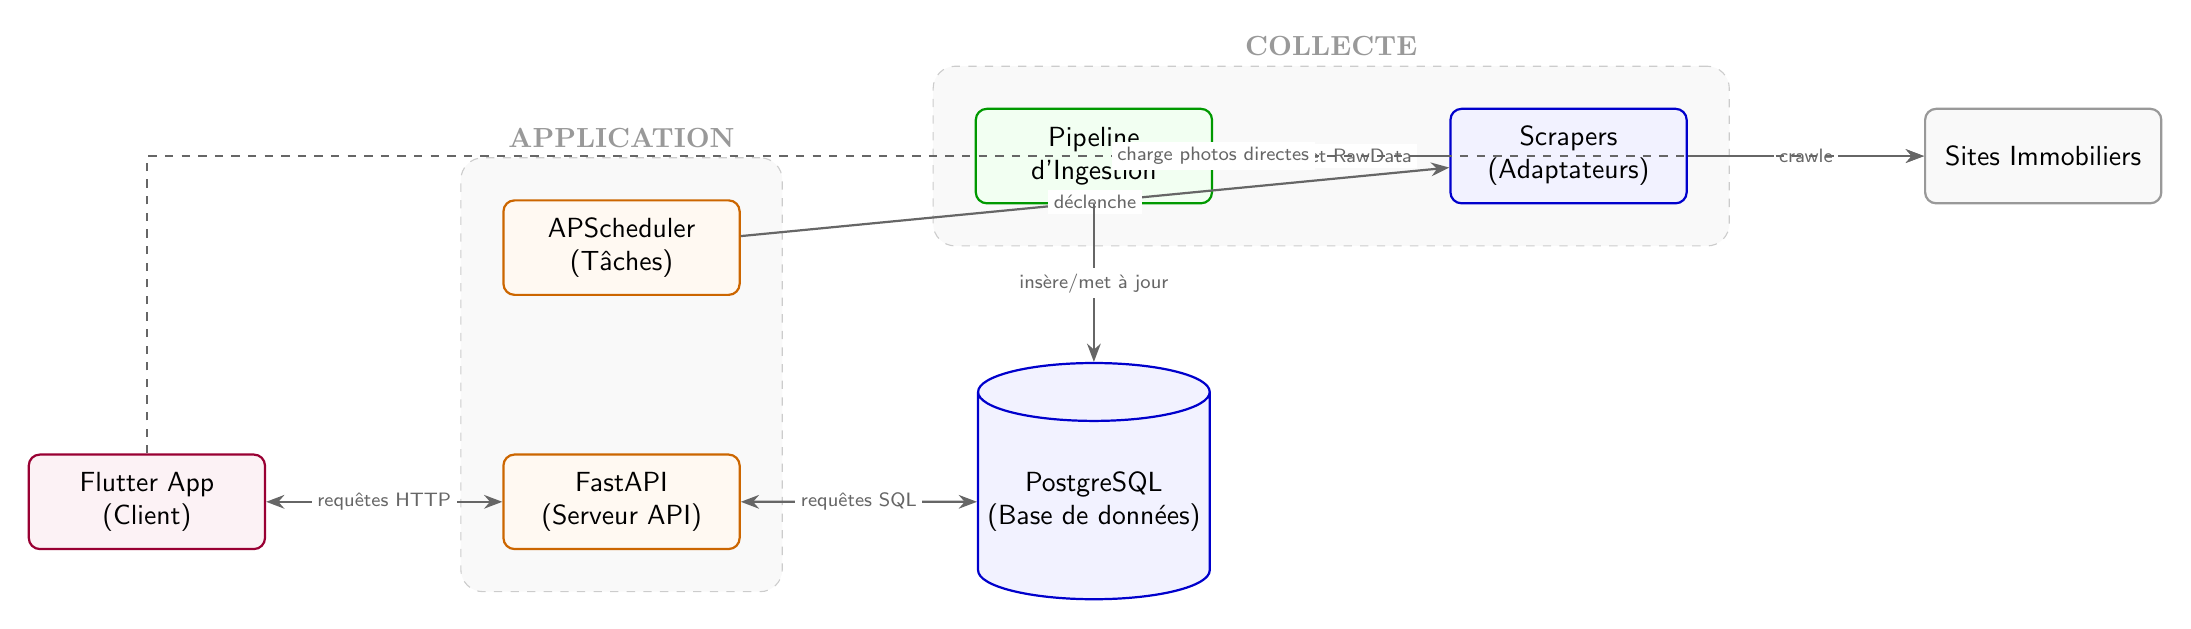
\begin{tikzpicture}[node distance=2cm and 3cm]

% Nodes
\node[comp, compPurple] (client) {Flutter App\\(Client)};
\node[comp, compOrange, right=of client] (api) {FastAPI\\(Serveur API)};
\node[comp, compOrange, above=of api] (sched) {APScheduler\\(Tâches)};
\node[db, right=of api] (db) {PostgreSQL\\(Base de données)};
\node[comp, compGreen, above=of db] (ingest) {Pipeline\\d'Ingestion};
\node[comp, compBlue, right=of ingest] (scrap) {Scrapers\\(Adaptateurs)};
\node[comp, draw=gray!80, fill=gray!5, right=of scrap] (web) {Sites Immobiliers};

% Background Groups
\begin{scope}[on background layer]
    \node[group, fit=(api)(sched), label={[font=\bfseries, text=gray!80]above:APPLICATION}] {};
    \node[group, fit=(scrap)(ingest), label={[font=\bfseries, text=gray!80]above:COLLECTE}] {};
\end{scope}

% Arrows
\draw[flow, <->] (client) -- node[lbl] {requêtes HTTP} (api);
\draw[flow, <->] (api) -- node[lbl] {requêtes SQL} (db);
\draw[flow] (sched) -- node[lbl] {déclenche} (scrap);
\draw[flow] (scrap) -- node[lbl] {crawle} (web);
\draw[flow] (scrap) -- node[lbl] {transmet RawData} (ingest);
\draw[flow] (ingest) -- node[lbl] {insère/met à jour} (db);
\draw[flow, dashed] (client) |- node[lbl, pos=0.8] {charge photos directes} (web);

\end{tikzpicture}
\end{center}

% ============================================================
% DIAGRAM 2 — DÉPLOIEMENT AWS
% ============================================================
\clearpage
\section*{Diagramme 2 — Déploiement AWS}
\begin{center}
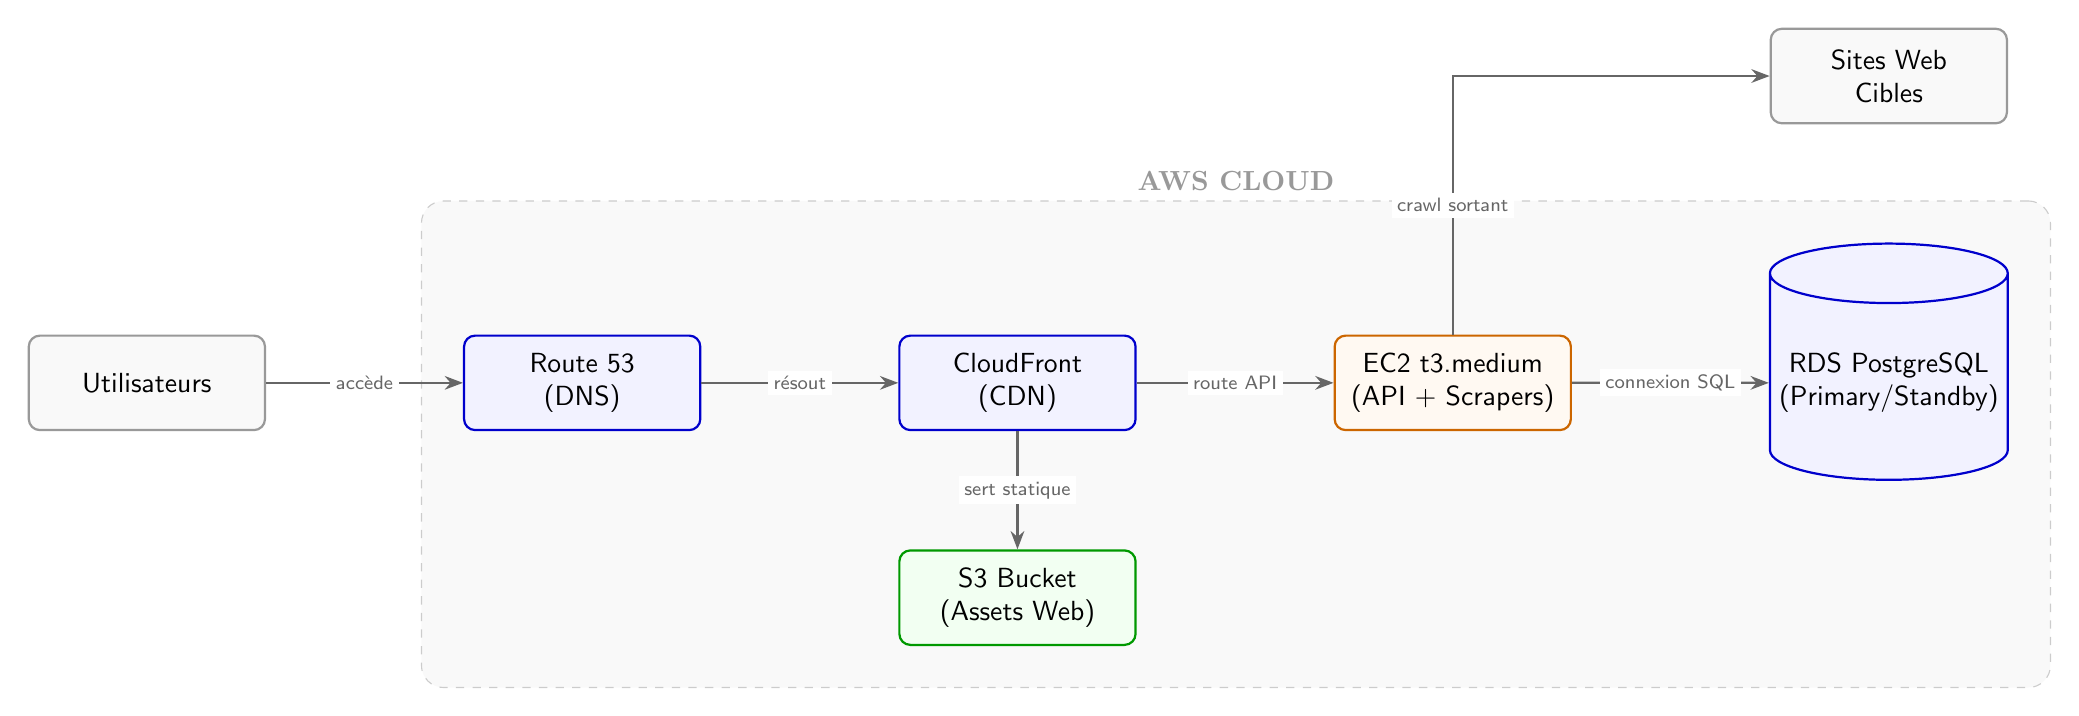
\begin{tikzpicture}[node distance=1.5cm and 2.5cm]

\node[comp, draw=gray!80, fill=gray!5] (users) {Utilisateurs};
\node[comp, compBlue, right=of users] (r53) {Route 53\\(DNS)};
\node[comp, compBlue, right=of r53] (cf) {CloudFront\\(CDN)};
\node[comp, compOrange, right=of cf] (ec2) {EC2 t3.medium\\(API + Scrapers)};
\node[db, right=of ec2] (rds) {RDS PostgreSQL\\(Primary/Standby)};

\node[comp, compGreen, below=of cf] (s3) {S3 Bucket\\(Assets Web)};
\node[comp, draw=gray!80, fill=gray!5, above=of rds] (sites) {Sites Web\\Cibles};

\draw[flow] (users) -- node[lbl] {accède} (r53);
\draw[flow] (r53) -- node[lbl] {résout} (cf);
\draw[flow] (cf) -- node[lbl] {route API} (ec2);
\draw[flow] (cf) -- node[lbl] {sert statique} (s3);
\draw[flow] (ec2) -- node[lbl] {connexion SQL} (rds);
\draw[flow] (ec2) |- node[lbl, near start] {crawl sortant} (sites);

\begin{scope}[on background layer]
    \node[group, fit=(r53)(cf)(ec2)(rds)(s3), label={[font=\bfseries, text=gray!80]above:AWS CLOUD}] {};
\end{scope}

\end{tikzpicture}
\end{center}

% ============================================================
% DIAGRAM 3 — MODÈLE DE DONNÉES (ER)
% ============================================================
\clearpage
\section*{Diagramme 3 — Modèle de Données (Relations Clés)}
\begin{center}
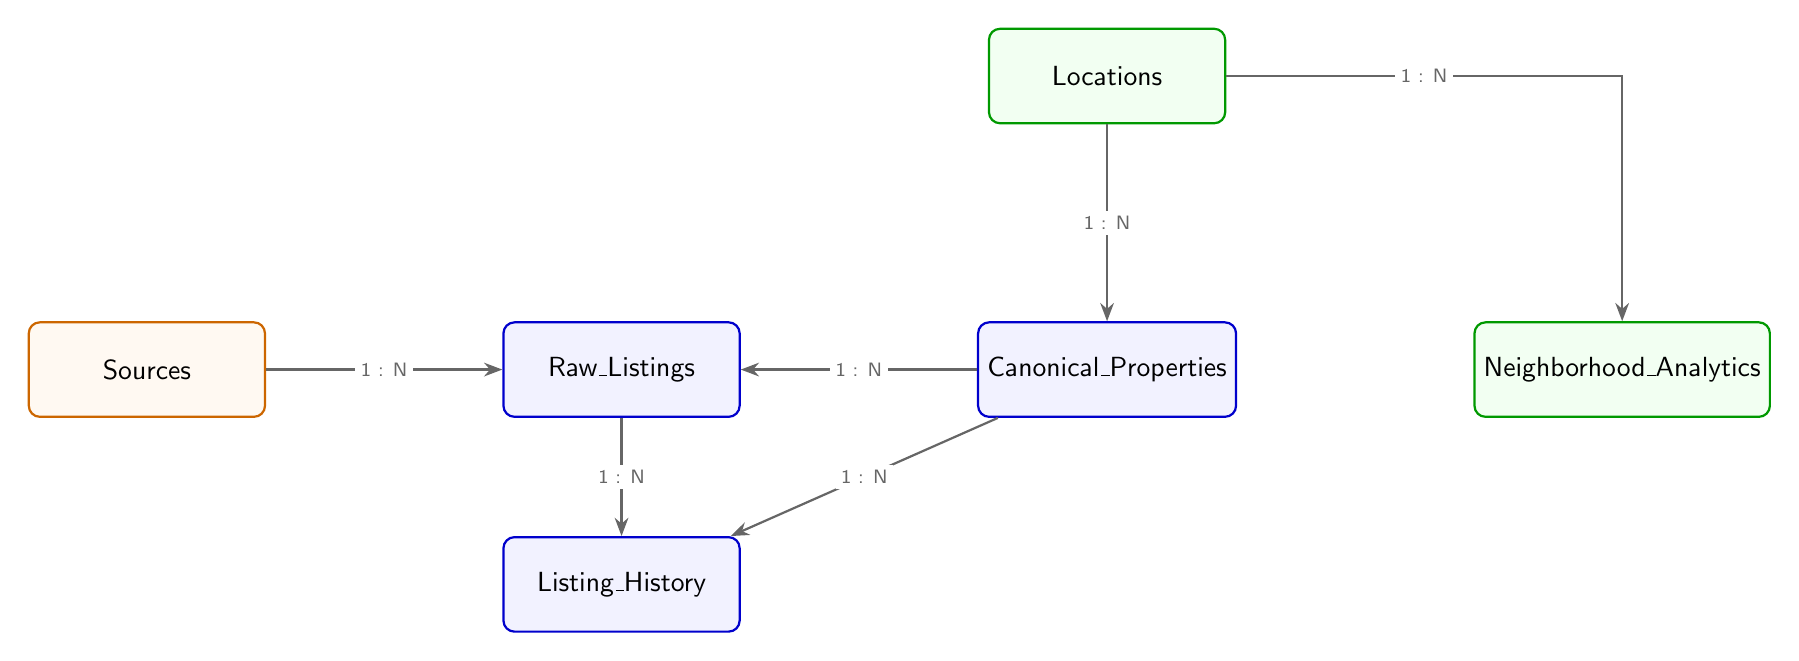
\begin{tikzpicture}[node distance=2.5cm and 3cm]

\node[comp, compOrange] (sources) {Sources};
\node[comp, compBlue, right=of sources] (raw) {Raw\_Listings};
\node[comp, compBlue, right=of raw] (canon) {Canonical\_Properties};
\node[comp, compGreen, above=of canon] (loc) {Locations};
\node[comp, compBlue, below=1.5cm of raw] (hist) {Listing\_History};
\node[comp, compGreen, right=of canon] (analyt) {Neighborhood\_Analytics};

\draw[flow] (sources) -- node[lbl] {1 : N} (raw);
\draw[flow] (canon) -- node[lbl] {1 : N} (raw);
\draw[flow] (canon) -- node[lbl] {1 : N} (hist);
\draw[flow] (raw) -- node[lbl] {1 : N} (hist);
\draw[flow] (loc) -- node[lbl] {1 : N} (canon);
\draw[flow] (loc) -| node[lbl, near start] {1 : N} (analyt);

\end{tikzpicture}
\end{center}

% ============================================================
% DIAGRAM 4 — FRAMEWORK DE SCRAPING
% ============================================================
\clearpage
\section*{Diagramme 4 — Framework de Scraping}
\begin{center}
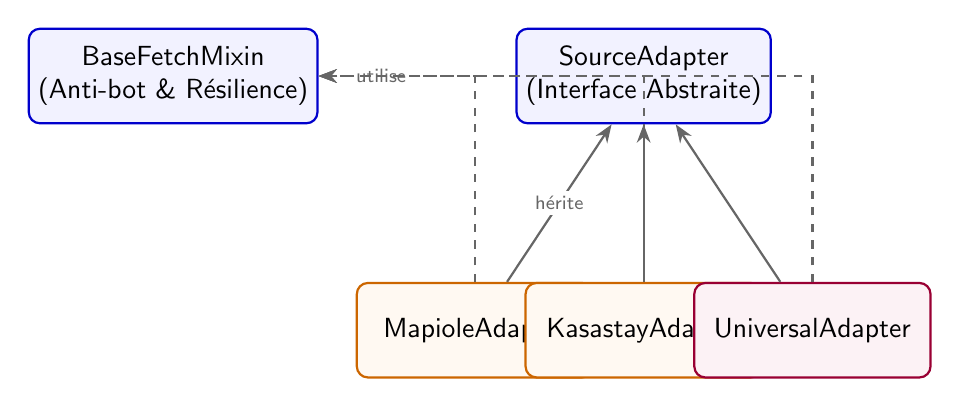
\begin{tikzpicture}[node distance=1.5cm and 2.5cm]

\node[comp, compBlue] (sabc) {SourceAdapter\\(Interface Abstraite)};
\node[comp, compBlue, left=of sabc] (bfm) {BaseFetchMixin\\(Anti-bot \& Résilience)};

\node[comp, compOrange, below left=2cm and -1cm of sabc] (mapi) {MapioleAdapter};
\node[comp, compOrange, below=2cm of sabc] (kasa) {KasastayAdapter};
\node[comp, compPurple, below right=2cm and -1cm of sabc] (univ) {UniversalAdapter};

\draw[flow, dashed] (mapi) |- node[lbl, pos=0.8] {utilise} (bfm);
\draw[flow, dashed] (kasa) |- (bfm);
\draw[flow, dashed] (univ) |- (bfm);

\draw[flow] (mapi) -- node[lbl] {hérite} (sabc);
\draw[flow] (kasa) -- (sabc);
\draw[flow] (univ) -- (sabc);

\end{tikzpicture}
\end{center}

% ============================================================
% DIAGRAM 5 — PIPELINE D'INGESTION
% ============================================================
\clearpage
\section*{Diagramme 5 — Pipeline d'Ingestion}
\begin{center}
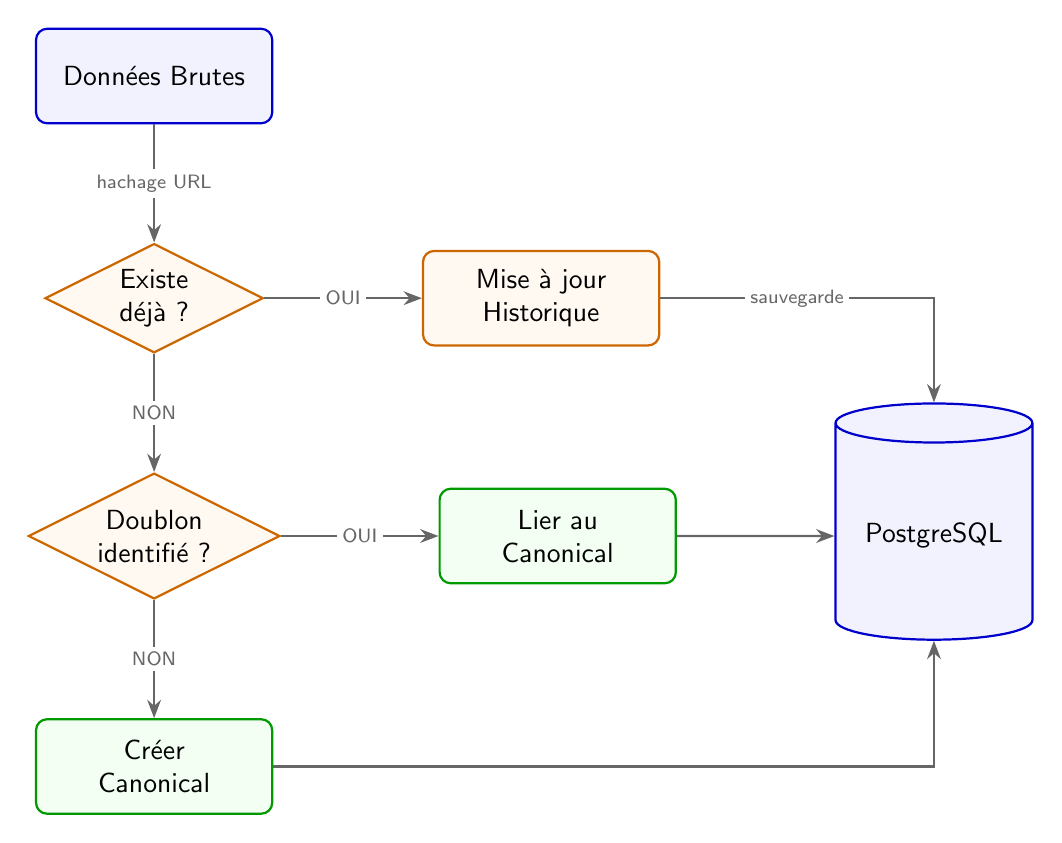
\begin{tikzpicture}[node distance=1.5cm and 2cm]

\node[comp, compBlue] (start) {Données Brutes};
\node[diamondShape, below=of start] (check) {Existe\\déjà ?};

\node[comp, compOrange, right=of check] (recrawl) {Mise à jour\\Historique};
\node[diamondShape, below=of check] (match) {Doublon\\identifié ?};

\node[comp, compGreen, right=of match] (link) {Lier au\\Canonical};
\node[comp, compGreen, below=of match] (create) {Créer\\Canonical};

\node[db, right=of link] (db) {PostgreSQL};

\draw[flow] (start) -- node[lbl] {hachage URL} (check);
\draw[flow] (check) -- node[lbl] {OUI} (recrawl);
\draw[flow] (check) -- node[lbl] {NON} (match);
\draw[flow] (match) -- node[lbl] {OUI} (link);
\draw[flow] (match) -- node[lbl] {NON} (create);

\draw[flow] (recrawl) -| node[lbl, near start] {sauvegarde} (db);
\draw[flow] (link) -- (db);
\draw[flow] (create) -| (db);

\end{tikzpicture}
\end{center}

% ============================================================
% DIAGRAM 6 — ORCHESTRATION DES CRAWLS
% ============================================================
\clearpage
\section*{Diagramme 6 — Orchestration des Crawls}
\begin{center}
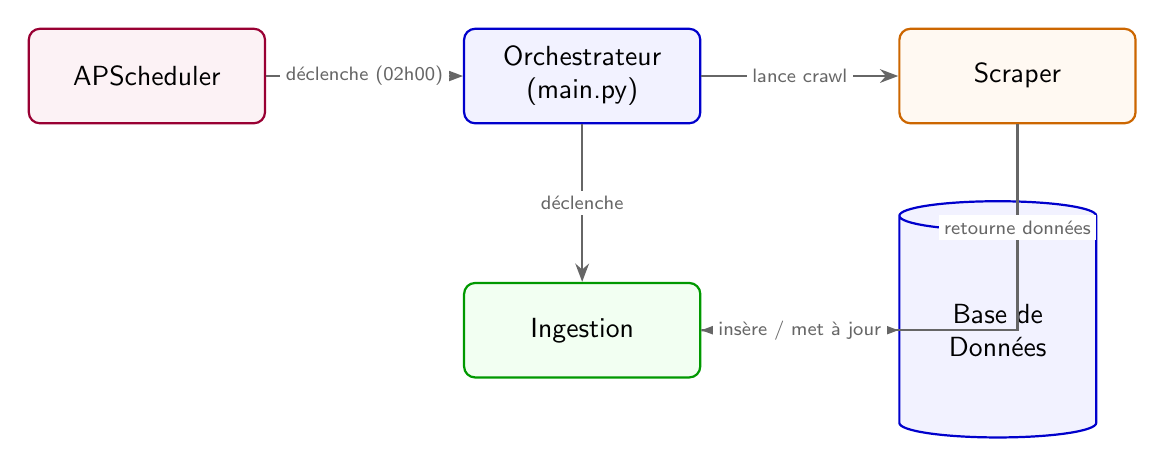
\begin{tikzpicture}[node distance=2cm and 2.5cm]

\node[comp, compPurple] (cron) {APScheduler};
\node[comp, compBlue, right=of cron] (main) {Orchestrateur\\(main.py)};
\node[comp, compOrange, right=of main] (scrap) {Scraper};
\node[comp, compGreen, below=of main] (ingest) {Ingestion};
\node[db, right=of ingest] (db) {Base de\\Données};

\draw[flow] (cron) -- node[lbl] {déclenche (02h00)} (main);
\draw[flow] (main) -- node[lbl] {lance crawl} (scrap);
\draw[flow] (scrap) |- node[lbl, near start] {retourne données} (ingest);
\draw[flow] (ingest) -- node[lbl] {insère / met à jour} (db);
\draw[flow] (main) -- node[lbl] {déclenche} (ingest);

\end{tikzpicture}
\end{center}

% ============================================================
% DIAGRAM 7 — RÉSOLUTION DES DOUBLONS (DCS)
% ============================================================
\clearpage
\section*{Diagramme 7 — Résolution des Doublons (DCS)}
\begin{center}
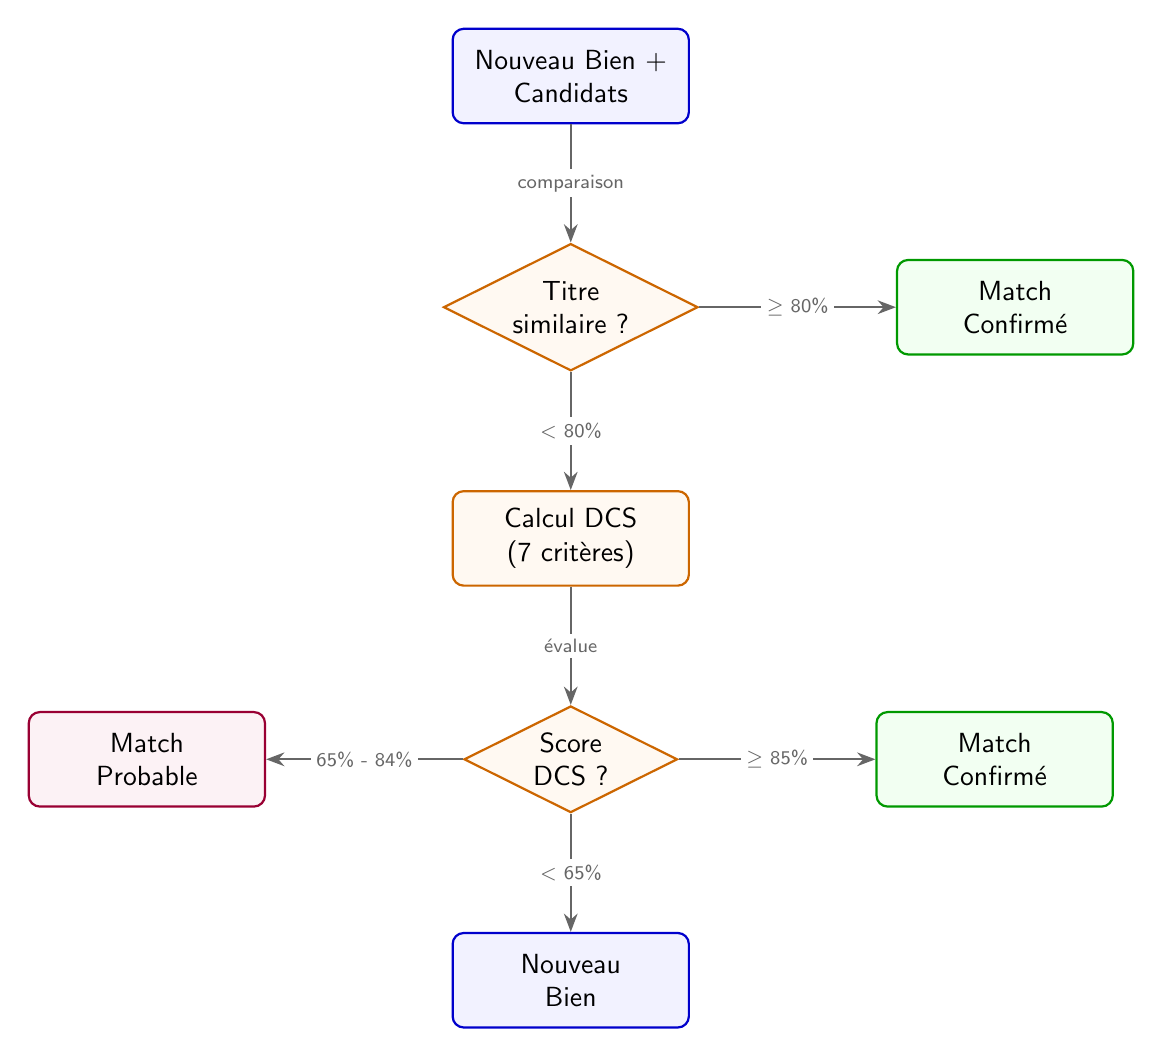
\begin{tikzpicture}[node distance=1.5cm and 2.5cm]

\node[comp, compBlue] (start) {Nouveau Bien +\\Candidats};
\node[diamondShape, below=of start] (sim) {Titre\\similaire ?};

\node[comp, compGreen, right=of sim] (conf1) {Match\\Confirmé};
\node[comp, compOrange, below=of sim] (dcs) {Calcul DCS\\(7 critères)};
\node[diamondShape, below=of dcs] (score) {Score\\DCS ?};

\node[comp, compGreen, right=of score] (conf2) {Match\\Confirmé};
\node[comp, compPurple, left=of score] (prob) {Match\\Probable};
\node[comp, compBlue, below=of score] (new) {Nouveau\\Bien};

\draw[flow] (start) -- node[lbl] {comparaison} (sim);
\draw[flow] (sim) -- node[lbl] {$\geq$ 80\%} (conf1);
\draw[flow] (sim) -- node[lbl] {$<$ 80\%} (dcs);
\draw[flow] (dcs) -- node[lbl] {évalue} (score);
\draw[flow] (score) -- node[lbl] {$\geq$ 85\%} (conf2);
\draw[flow] (score) -- node[lbl] {65\% - 84\%} (prob);
\draw[flow] (score) -- node[lbl] {$<$ 65\%} (new);

\end{tikzpicture}
\end{center}

% ============================================================
% DIAGRAM 8 — SCRAPER UNIVERSEL (4 ÉTAPES)
% ============================================================
\clearpage
\section*{Diagramme 8 — Scraper Universel}
\begin{center}
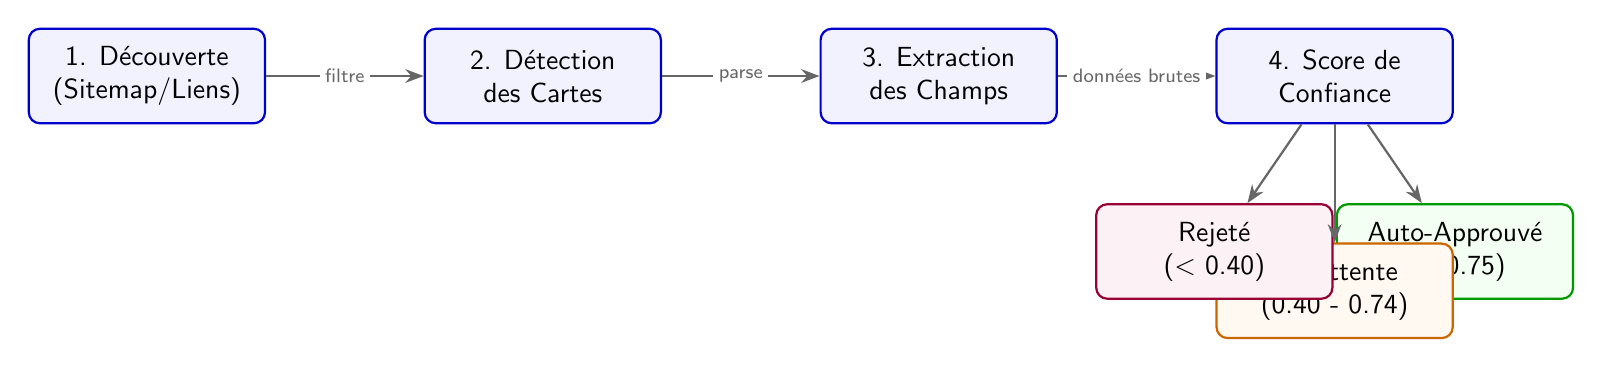
\begin{tikzpicture}[node distance=1.5cm and 2cm]

\node[comp, compBlue] (e1) {1. Découverte\\(Sitemap/Liens)};
\node[comp, compBlue, right=of e1] (e2) {2. Détection\\des Cartes};
\node[comp, compBlue, right=of e2] (e3) {3. Extraction\\des Champs};
\node[comp, compBlue, right=of e3] (e4) {4. Score de\\Confiance};

\node[comp, compGreen, below right=1cm and -1.5cm of e4] (ok) {Auto-Approuvé\\($\geq$ 0.75)};
\node[comp, compOrange, below=of e4] (wait) {En Attente\\(0.40 - 0.74)};
\node[comp, compPurple, below left=1cm and -1.5cm of e4] (rej) {Rejeté\\($<$ 0.40)};

\draw[flow] (e1) -- node[lbl] {filtre} (e2);
\draw[flow] (e2) -- node[lbl] {parse} (e3);
\draw[flow] (e3) -- node[lbl] {données brutes} (e4);
\draw[flow] (e4) -- (ok);
\draw[flow] (e4) -- (wait);
\draw[flow] (e4) -- (rej);

\end{tikzpicture}
\end{center}

% ============================================================
% DIAGRAM 9 — PIPELINE ANALYTIQUE
% ============================================================
\clearpage
\section*{Diagramme 9 — Pipeline Analytique}
\begin{center}
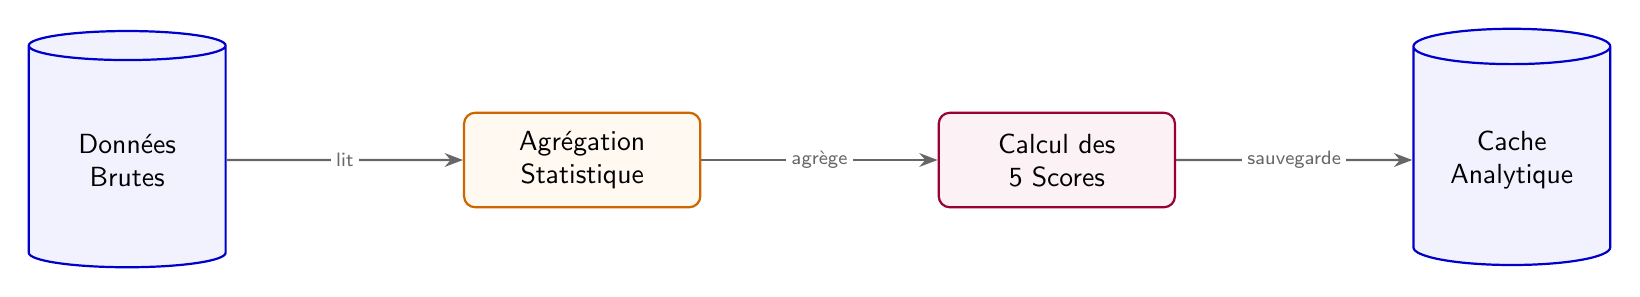
\begin{tikzpicture}[node distance=2cm and 3cm]

\node[db] (in) {Données\\Brutes};
\node[comp, compOrange, right=of in] (agg) {Agrégation\\Statistique};
\node[comp, compPurple, right=of agg] (scores) {Calcul des\\5 Scores};
\node[db, right=of scores] (out) {Cache\\Analytique};

\draw[flow] (in) -- node[lbl] {lit} (agg);
\draw[flow] (agg) -- node[lbl] {agrège} (scores);
\draw[flow] (scores) -- node[lbl] {sauvegarde} (out);

\end{tikzpicture}
\end{center}

% ============================================================
% DIAGRAM 10 — FLUX DE REQUÊTES API
% ============================================================
\clearpage
\section*{Diagramme 10 — Flux de Requêtes API}
\begin{center}
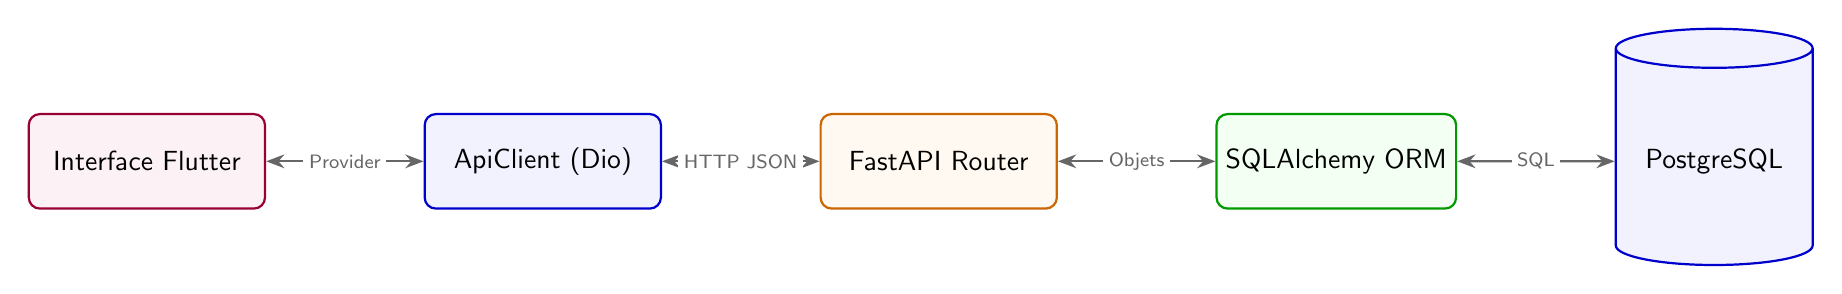
\begin{tikzpicture}[node distance=2cm and 2cm]

\node[comp, compPurple] (ui) {Interface Flutter};
\node[comp, compBlue, right=of ui] (dio) {ApiClient (Dio)};
\node[comp, compOrange, right=of dio] (api) {FastAPI Router};
\node[comp, compGreen, right=of api] (orm) {SQLAlchemy ORM};
\node[db, right=of orm] (db) {PostgreSQL};

\draw[flow, <->] (ui) -- node[lbl] {Provider} (dio);
\draw[flow, <->] (dio) -- node[lbl] {HTTP JSON} (api);
\draw[flow, <->] (api) -- node[lbl] {Objets} (orm);
\draw[flow, <->] (orm) -- node[lbl] {SQL} (db);

\end{tikzpicture}
\end{center}

% ============================================================
% DIAGRAM 11 — MACHINE À ÉTATS DU REVIEW
% ============================================================
\clearpage
\section*{Diagramme 11 — Machine à États (Validation)}
\begin{center}
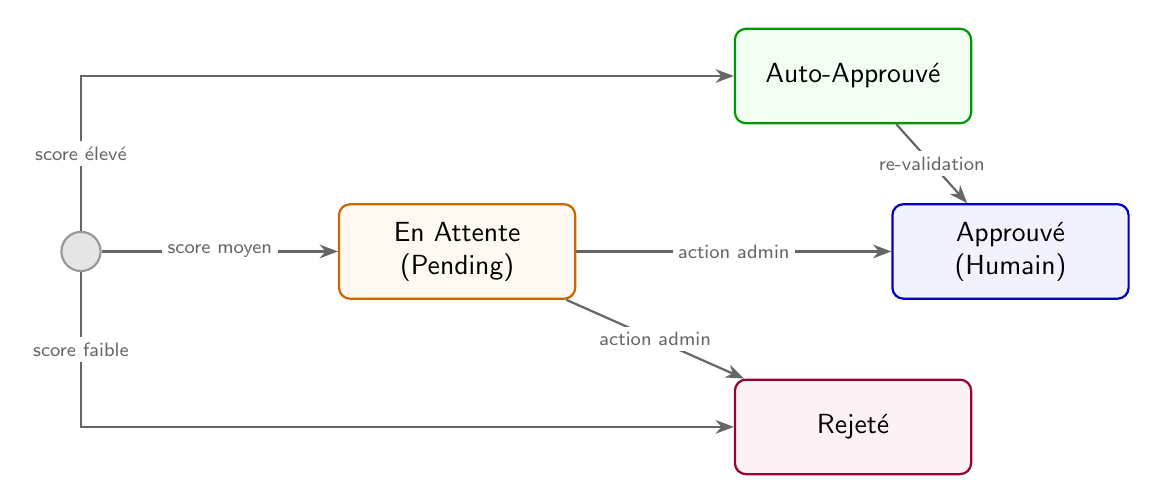
\begin{tikzpicture}[node distance=2.5cm and 3cm]

\node[circle, draw=gray!80, fill=gray!20, thick, inner sep=5pt] (start) {};
\node[comp, compOrange, right=of start] (pend) {En Attente\\(Pending)};
\node[comp, compGreen, above right=1cm and 2cm of pend] (auto) {Auto-Approuvé};
\node[comp, compPurple, below right=1cm and 2cm of pend] (rej) {Rejeté};
\node[comp, compBlue, right=4cm of pend] (hum) {Approuvé\\(Humain)};

\draw[flow] (start) -- node[lbl] {score moyen} (pend);
\draw[flow] (start) |- node[lbl, near start] {score élevé} (auto);
\draw[flow] (start) |- node[lbl, near start] {score faible} (rej);

\draw[flow] (pend) -- node[lbl] {action admin} (hum);
\draw[flow] (pend) -- node[lbl] {action admin} (rej);
\draw[flow] (auto) -- node[lbl] {re-validation} (hum);

\end{tikzpicture}
\end{center}

% ============================================================
% DIAGRAM S1 — MOTEUR DE SCRAPING
% ============================================================
\clearpage
\section*{Diagramme S1 — Le Moteur de Scraping}
\begin{center}
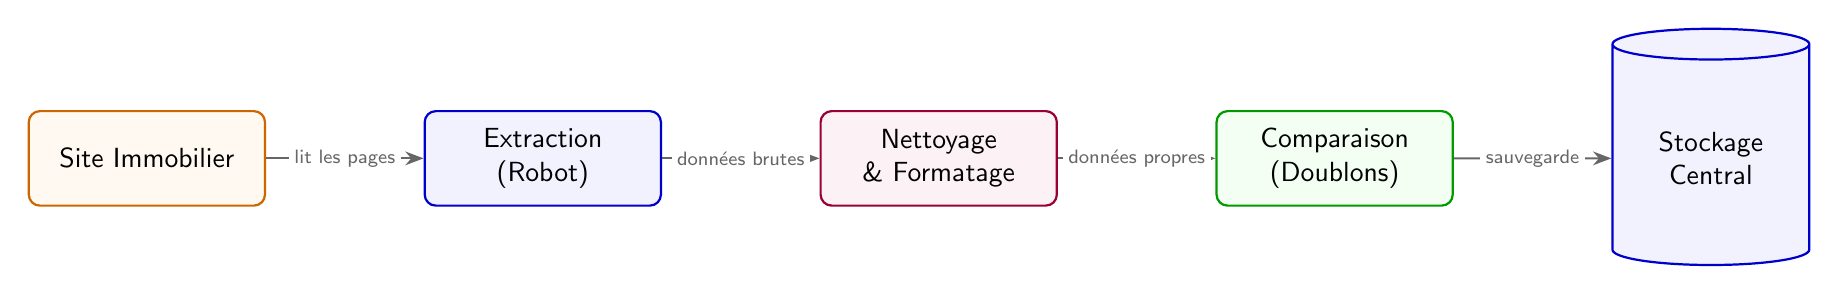
\begin{tikzpicture}[node distance=1.5cm and 2cm]

\node[comp, compOrange] (site) {Site Immobilier};
\node[comp, compBlue, right=of site] (extr) {Extraction\\(Robot)};
\node[comp, compPurple, right=of extr] (clean) {Nettoyage\\\& Formatage};
\node[comp, compGreen, right=of clean] (comp) {Comparaison\\(Doublons)};
\node[db, right=of comp] (db) {Stockage\\Central};

\draw[flow] (site) -- node[lbl] {lit les pages} (extr);
\draw[flow] (extr) -- node[lbl] {données brutes} (clean);
\draw[flow] (clean) -- node[lbl] {données propres} (comp);
\draw[flow] (comp) -- node[lbl] {sauvegarde} (db);

\end{tikzpicture}
\end{center}

% ============================================================
% DIAGRAM S2 — ARCHITECTURE GLOBALE
% ============================================================
\clearpage
\section*{Diagramme S2 — Architecture Globale}
\begin{center}
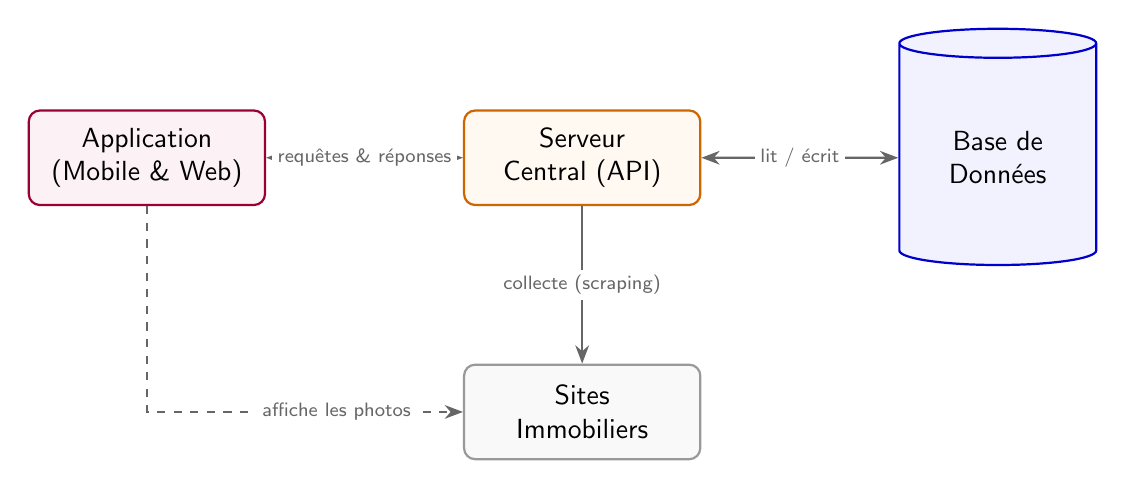
\begin{tikzpicture}[node distance=2cm and 2.5cm]

\node[comp, compPurple] (app) {Application\\(Mobile \& Web)};
\node[comp, compOrange, right=of app] (srv) {Serveur\\Central (API)};
\node[db, right=of srv] (db) {Base de\\Données};
\node[comp, draw=gray!80, fill=gray!5, below=of srv] (web) {Sites\\Immobiliers};

\draw[flow, <->] (app) -- node[lbl] {requêtes \& réponses} (srv);
\draw[flow, <->] (srv) -- node[lbl] {lit / écrit} (db);
\draw[flow] (srv) -- node[lbl] {collecte (scraping)} (web);
\draw[flow, dashed] (app) |- node[lbl, pos=0.8] {affiche les photos} (web);

\end{tikzpicture}
\end{center}

% ============================================================
% DIAGRAM S3 — USE CASE RECHERCHE
% ============================================================
\clearpage
\section*{Diagramme S3 — Scénario: Recherche}
\begin{center}
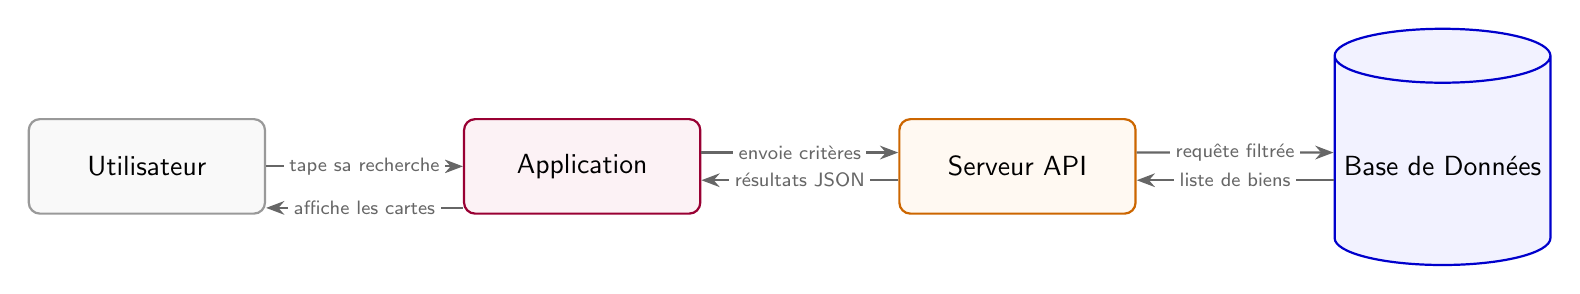
\begin{tikzpicture}[node distance=2cm and 2.5cm]

\node[comp, draw=gray!80, fill=gray!5] (user) {Utilisateur};
\node[comp, compPurple, right=of user] (app) {Application};
\node[comp, compOrange, right=of app] (srv) {Serveur API};
\node[db, right=of srv] (db) {Base de Données};

\draw[flow] (user) -- node[lbl] {tape sa recherche} (app);
\draw[flow, transform canvas={yshift=5pt}] (app) -- node[lbl] {envoie critères} (srv);
\draw[flow, transform canvas={yshift=5pt}] (srv) -- node[lbl] {requête filtrée} (db);
\draw[flow, transform canvas={yshift=-5pt}] (db) -- node[lbl] {liste de biens} (srv);
\draw[flow, transform canvas={yshift=-5pt}] (srv) -- node[lbl] {résultats JSON} (app);
\draw[flow, transform canvas={yshift=-15pt}] (app) -- node[lbl] {affiche les cartes} (user);

\end{tikzpicture}
\end{center}

% ============================================================
% DIAGRAM S4 — USE CASE DÉTAIL BIEN
% ============================================================
\clearpage
\section*{Diagramme S4 — Scénario: Détail d'un Bien}
\begin{center}
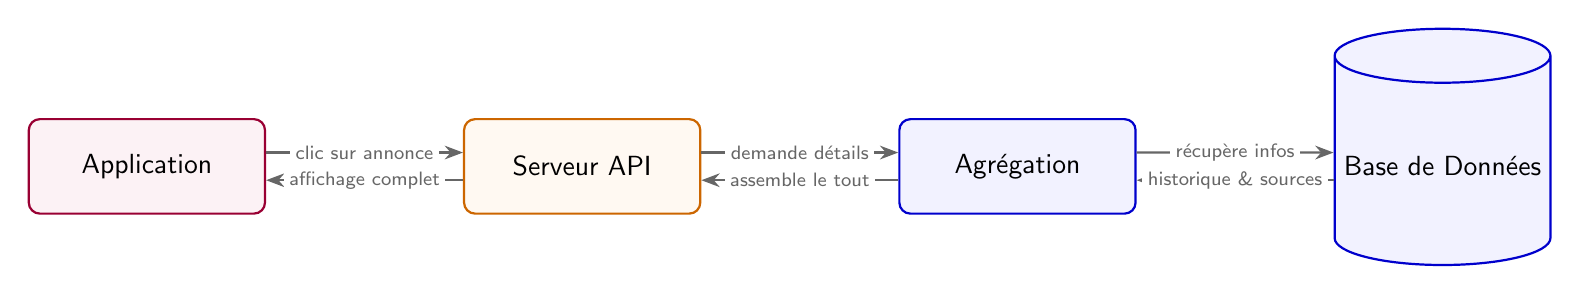
\begin{tikzpicture}[node distance=2cm and 2.5cm]

\node[comp, compPurple] (app) {Application};
\node[comp, compOrange, right=of app] (srv) {Serveur API};
\node[comp, compBlue, right=of srv] (agg) {Agrégation};
\node[db, right=of agg] (db) {Base de Données};

\draw[flow, transform canvas={yshift=5pt}] (app) -- node[lbl] {clic sur annonce} (srv);
\draw[flow, transform canvas={yshift=5pt}] (srv) -- node[lbl] {demande détails} (agg);
\draw[flow, transform canvas={yshift=5pt}] (agg) -- node[lbl] {récupère infos} (db);

\draw[flow, transform canvas={yshift=-5pt}] (db) -- node[lbl] {historique \& sources} (agg);
\draw[flow, transform canvas={yshift=-5pt}] (agg) -- node[lbl] {assemble le tout} (srv);
\draw[flow, transform canvas={yshift=-5pt}] (srv) -- node[lbl] {affichage complet} (app);

\end{tikzpicture}
\end{center}

% ============================================================
% DIAGRAM S5 — ÉVITER LES DOUBLONS
% ============================================================
\clearpage
\section*{Diagramme S5 — Comment éviter les Doublons}
\begin{center}
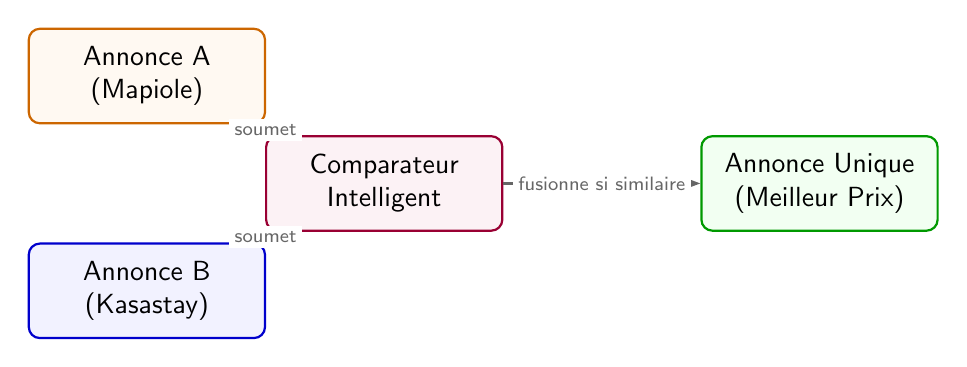
\begin{tikzpicture}[node distance=1.5cm and 2.5cm]

\node[comp, compOrange] (a1) {Annonce A\\(Mapiole)};
\node[comp, compBlue, below=of a1] (a2) {Annonce B\\(Kasastay)};
\node[comp, compPurple, right=1.5cm of $(a1)!0.5!(a2)$] (comp) {Comparateur\\Intelligent};
\node[comp, compGreen, right=of comp] (final) {Annonce Unique\\(Meilleur Prix)};

\draw[flow] (a1) -- node[lbl] {soumet} (comp);
\draw[flow] (a2) -- node[lbl] {soumet} (comp);
\draw[flow] (comp) -- node[lbl] {fusionne si similaire} (final);

\end{tikzpicture}
\end{center}

% ============================================================
% DIAGRAM S6 — SUIVI DES PRIX
% ============================================================
\clearpage
\section*{Diagramme S6 — Le Suivi des Prix dans le Temps}
\begin{center}
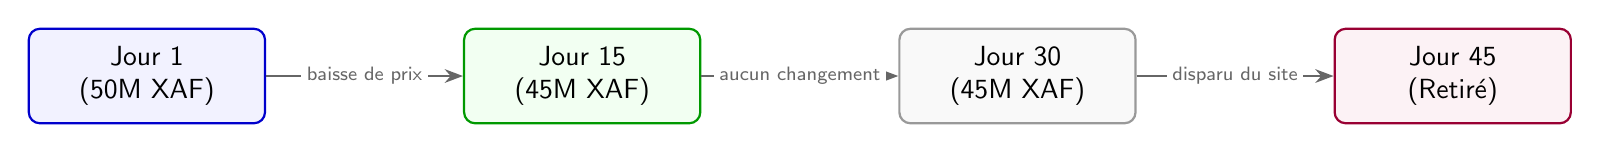
\begin{tikzpicture}[node distance=1.5cm and 2.5cm]

\node[comp, compBlue] (j1) {Jour 1\\(50M XAF)};
\node[comp, compGreen, right=of j1] (j15) {Jour 15\\(45M XAF)};
\node[comp, draw=gray!80, fill=gray!5, right=of j15] (j30) {Jour 30\\(45M XAF)};
\node[comp, compPurple, right=of j30] (j45) {Jour 45\\(Retiré)};

\draw[flow] (j1) -- node[lbl] {baisse de prix} (j15);
\draw[flow] (j15) -- node[lbl] {aucun changement} (j30);
\draw[flow] (j30) -- node[lbl] {disparu du site} (j45);

\end{tikzpicture}
\end{center}

% ============================================================
% DIAGRAM S7 — INTELLIGENCE QUARTIER
% ============================================================
\clearpage
\section*{Diagramme S7 — L'Intelligence du Quartier}
\begin{center}
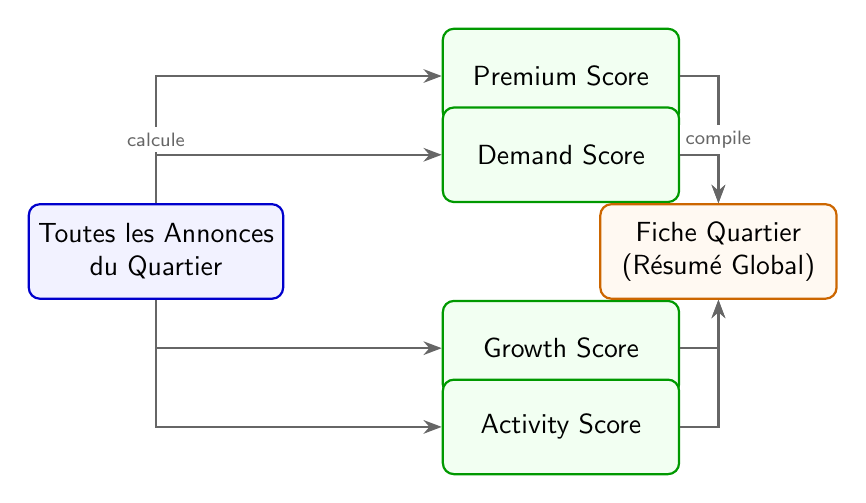
\begin{tikzpicture}[node distance=2cm and 2.5cm]

\node[comp, compBlue] (raw) {Toutes les Annonces\\du Quartier};

\node[comp, compGreen, above right=1cm and 2cm of raw] (s1) {Premium Score};
\node[comp, compGreen, above right=0cm and 2cm of raw] (s2) {Demand Score};
\node[comp, compGreen, below right=0cm and 2cm of raw] (s3) {Growth Score};
\node[comp, compGreen, below right=1cm and 2cm of raw] (s4) {Activity Score};

\node[comp, compOrange, right=4cm of raw] (fiche) {Fiche Quartier\\(Résumé Global)};

\draw[flow] (raw) |- node[lbl, near start] {calcule} (s1);
\draw[flow] (raw) |- (s2);
\draw[flow] (raw) |- (s3);
\draw[flow] (raw) |- (s4);

\draw[flow] (s1) -| node[lbl, near end] {compile} (fiche);
\draw[flow] (s2) -| (fiche);
\draw[flow] (s3) -| (fiche);
\draw[flow] (s4) -| (fiche);

\end{tikzpicture}
\end{center}

% ============================================================
% DIAGRAM S8 — CYCLE AUTOMATIQUE
% ============================================================
\clearpage
\section*{Diagramme S8 — Le Cycle Automatique}
\begin{center}
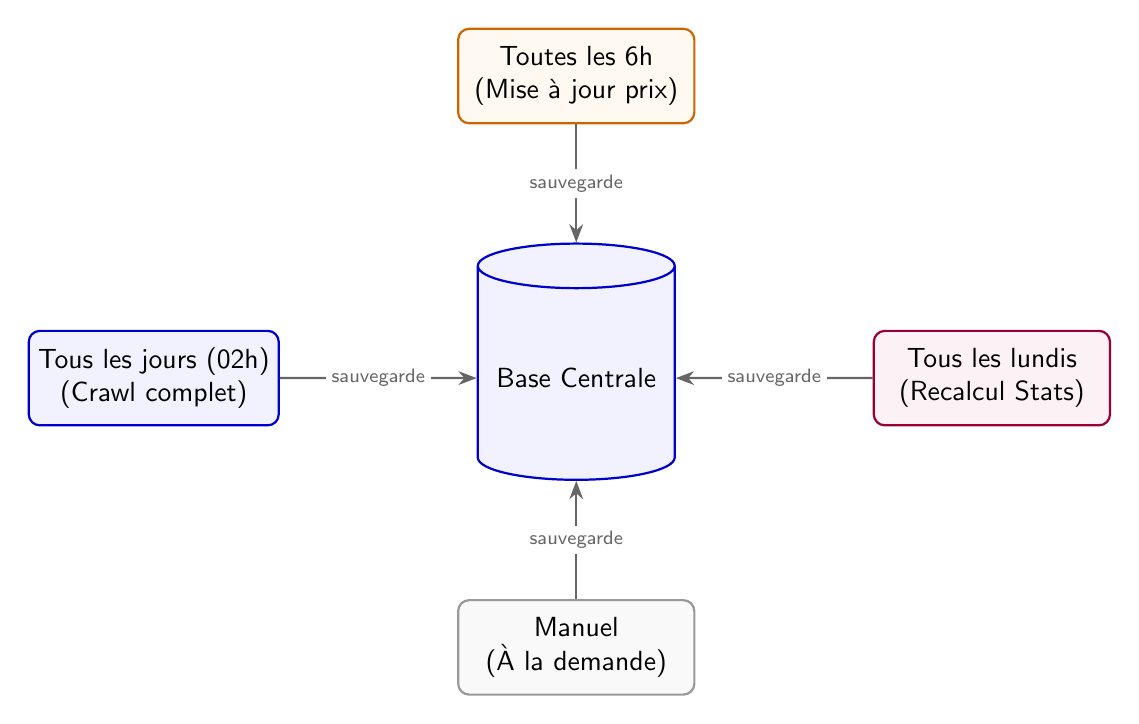
\begin{tikzpicture}[node distance=1.5cm and 2.5cm]

\node[db] (db) {Base Centrale};

\node[comp, compOrange, above=of db] (t1) {Toutes les 6h\\(Mise à jour prix)};
\node[comp, compBlue, left=of db] (t2) {Tous les jours (02h)\\(Crawl complet)};
\node[comp, compPurple, right=of db] (t3) {Tous les lundis\\(Recalcul Stats)};
\node[comp, draw=gray!80, fill=gray!5, below=of db] (t4) {Manuel\\(À la demande)};

\draw[flow] (t1) -- node[lbl] {sauvegarde} (db);
\draw[flow] (t2) -- node[lbl] {sauvegarde} (db);
\draw[flow] (t3) -- node[lbl] {sauvegarde} (db);
\draw[flow] (t4) -- node[lbl] {sauvegarde} (db);

\end{tikzpicture}
\end{center}

% ============================================================
% DIAGRAM S9 — AJOUTER UN NOUVEAU SITE
% ============================================================
\clearpage
\section*{Diagramme S9 — Ajouter un Nouveau Site}
\begin{center}
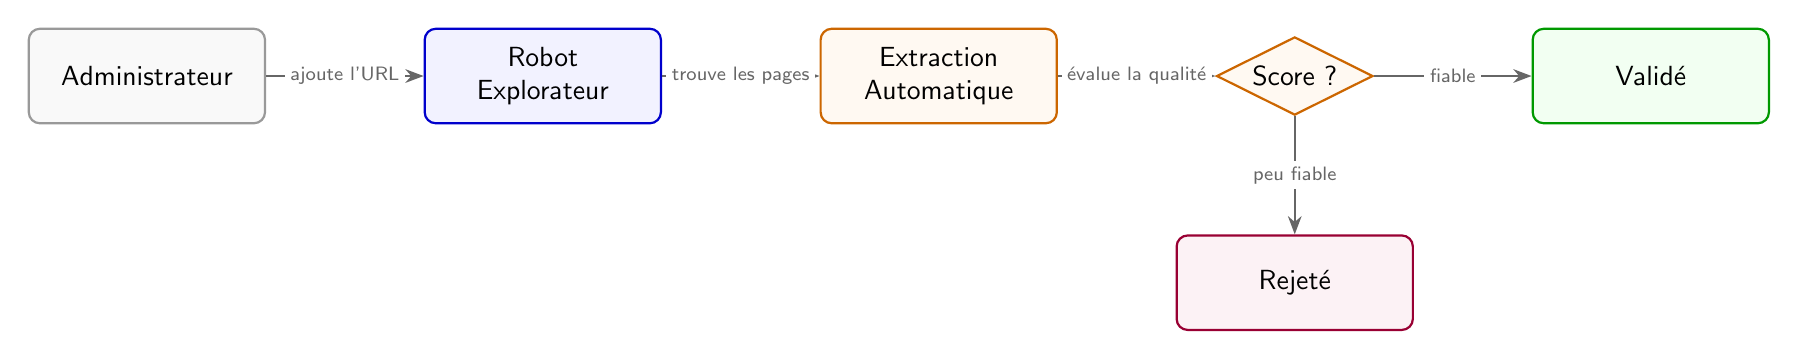
\begin{tikzpicture}[node distance=1.5cm and 2cm]

\node[comp, draw=gray!80, fill=gray!5] (admin) {Administrateur};
\node[comp, compBlue, right=of admin] (robot) {Robot\\Explorateur};
\node[comp, compOrange, right=of robot] (extr) {Extraction\\Automatique};
\node[diamondShape, right=of extr] (score) {Score ?};

\node[comp, compGreen, right=of score] (ok) {Validé};
\node[comp, compPurple, below=of score] (rej) {Rejeté};

\draw[flow] (admin) -- node[lbl] {ajoute l'URL} (robot);
\draw[flow] (robot) -- node[lbl] {trouve les pages} (extr);
\draw[flow] (extr) -- node[lbl] {évalue la qualité} (score);
\draw[flow] (score) -- node[lbl] {fiable} (ok);
\draw[flow] (score) -- node[lbl] {peu fiable} (rej);

\end{tikzpicture}
\end{center}

% ============================================================
% DIAGRAM S10 — GESTION DES IMAGES
% ============================================================
\clearpage
\section*{Diagramme S10 — Gestion des Images}
\begin{center}
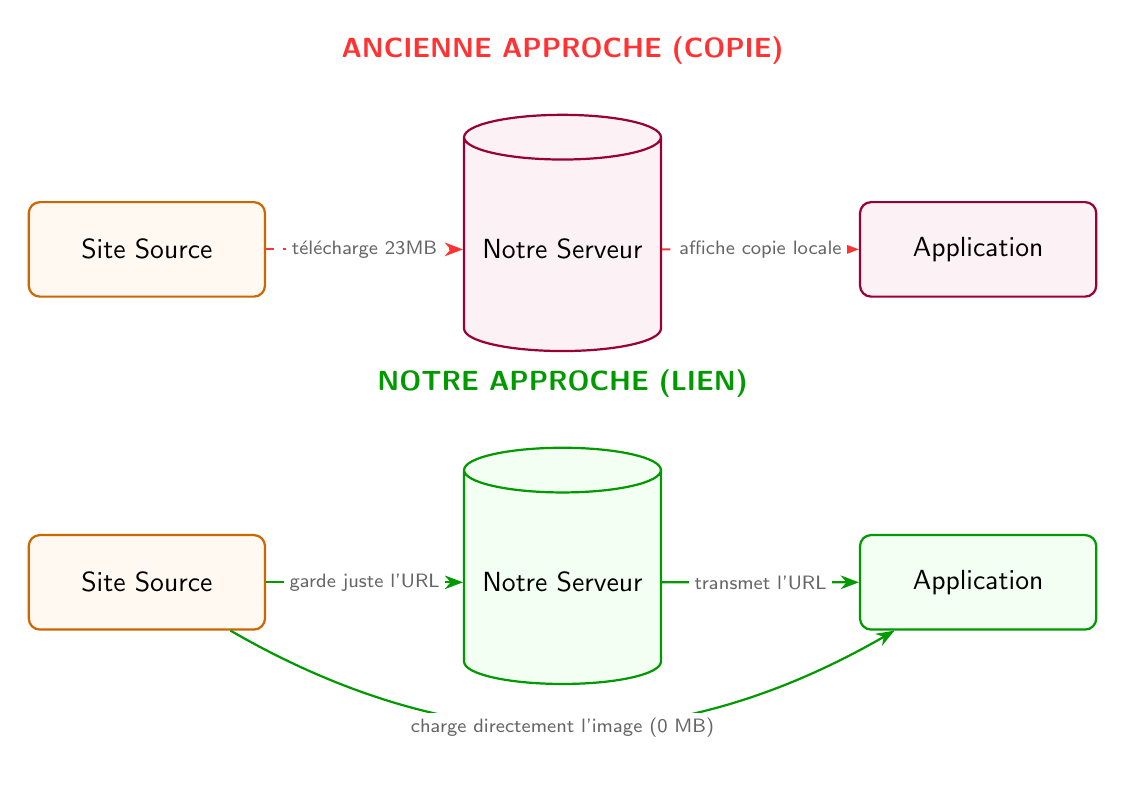
\begin{tikzpicture}[node distance=2.5cm and 2.5cm]

% Mauvaise approche
\node[comp, compOrange] (s1) {Site Source};
\node[db, compPurple, right=of s1] (db1) {Notre Serveur};
\node[comp, compPurple, right=of db1] (app1) {Application};

\draw[flow, dashed, draw=red!80] (s1) -- node[lbl] {télécharge 23MB} (db1);
\draw[flow, dashed, draw=red!80] (db1) -- node[lbl] {affiche copie locale} (app1);

\node[above=0.5cm of db1, font=\bfseries\sffamily, text=red!80] {ANCIENNE APPROCHE (COPIE)};

% Bonne approche
\node[comp, compOrange, below=3cm of s1] (s2) {Site Source};
\node[db, compGreen, right=of s2] (db2) {Notre Serveur};
\node[comp, compGreen, right=of db2] (app2) {Application};

\draw[flow, draw=green!60!black] (s2) -- node[lbl] {garde juste l'URL} (db2);
\draw[flow, draw=green!60!black] (db2) -- node[lbl] {transmet l'URL} (app2);
\draw[flow, draw=green!60!black, bend right=30] (s2) to node[lbl, swap] {charge directement l'image (0 MB)} (app2);

\node[above=0.5cm of db2, font=\bfseries\sffamily, text=green!60!black] {NOTRE APPROCHE (LIEN)};

\end{tikzpicture}
\end{center}

\end{document}
